\documentclass[conference]{IEEEtran}

\usepackage{amsmath}
\usepackage{url}
\usepackage{cite}
\usepackage{graphicx}


% correct bad hyphenation here
% \hyphenation{op-tical net-works semi-conduc-tor}


\begin{document}

\title{Generation T --- Pronounceable Password Generation Gamified\\
CPEN 442 Project Proposal}


% author names and affiliations
% use a multiple column layout for up to three different
% affiliations
% % % % CHANGE: Add your aliases here
\author{\IEEEauthorblockN{blue, v6q8}
\IEEEauthorblockA{Department of Computer Science\\
University of British Columbia\\
}
\and
\IEEEauthorblockN{Matt Labbe, hydro}
\IEEEauthorblockA{Electrical and\\Computer Engineering\\
University of British Columbia\\
}
}


% make the title area
\maketitle

% As a general rule, do not put math, special symbols or citations
% in the abstract
\begin{abstract}
A study in gamified password generation is considered. The central idea is an extension on the memorability of pronounceable passwords. We use gamification as a means of introducing \emph{choice} and \emph{interaction} in near random generation of pronounceable passwords.
\end{abstract}

\section{Introduction}
% no \IEEEPARstart
Despite the plentiful amount of work on passwords done by the information security community, it remains an open issue. Secure and sufficiently unpredictable passwords are seemingly incompatible with their human counterparts, who will be the primary agents actively generating and using them. It is generally known that the more memorable the password, the more easily it will be compromised, since they rely on tricks such as passphrases and mnemonics, which allow them to be easily guessed using attacks such as a combinatorial attack. Further, it is ideal that users employ different passwords for each account they may use. Thus, we focus on the memorability of pronouncable passwords using a gamified generation approach. \emph{Gamification} is easily summarized as masking a primary, usually important or useful, but tedious or difficult, task while leveraging some specially designed leisurely or enjoyable task. Using this approach we want to investigate the role of interaction and choice on memorability in the hopes that longer, and thus more secure, passwords can be generated that remain useable. The system we designed will most likely be used to complement existing password aids such as password managers where, regardless of its ability to store and proffer passwords when needed, users must still memorize at least one password. The hope is that this particular password is memorable, as unpredictable as possible and stored locally on client hardware 
% or, for more savvy users, backed up safely for retreival
.

\section{Related Works}
We first caught the inspiration to use \emph{atomic} fragments of language called phonemes from \cite{proposal:phonemes}. This resource also provided some phoneme sets such as the consonant sounds {\tt b, c, d, f, g, h, j, k, l, m, n, p, r, s, t, v, w, x, y, z, bl, br, dr, ch, cr, dr, fl, fr, gr, gl, pl, pr, qu, sh, sl, sp, st, sw, th, tr} concatenated with a vowel sound following. This lead quickly to the idea of actions deriving substrings as needed in a gamified task. Next, we considered some heuristics to determine and measure prounounceability in \cite{proposal:prounounceability} which will be useful in scoring putative passwords and possibly influence the assignment of phonemes to blocks. Finally, we consider the alternative of mnemonic password derivation in \cite{proposal:mnemonic} as well as the evaluation design.

\section{Proposed Approach}
We attempt to modify the popular game \emph{Tetris} since we consider its mechanics are well known by users of computing devices and thus the procedure will be nearly self explanatory. The modifications reside in the encoding of phonemes which are randomly assigned to each block (refer to figure \ref{tet}) of a tetromino. As lines are cleared, the phonemes associated to the blocks involved in the lines construct putative strings which will then be ranked and suggested to the user. We believe that this approximates a random process: the blocks are given random phonemes and the user, in playing the game offers another source of entropy. However, the principle interest lies in the latter---does the user's interaction with this system afford better memorability than a fully automated random process? It is convincing that ultimately passwords should be memorable if they are to be secure, since if long passwords remain memorable, we can in principle construct arbitrarily long passwords that retain usability.
\begin{figure}[t]
	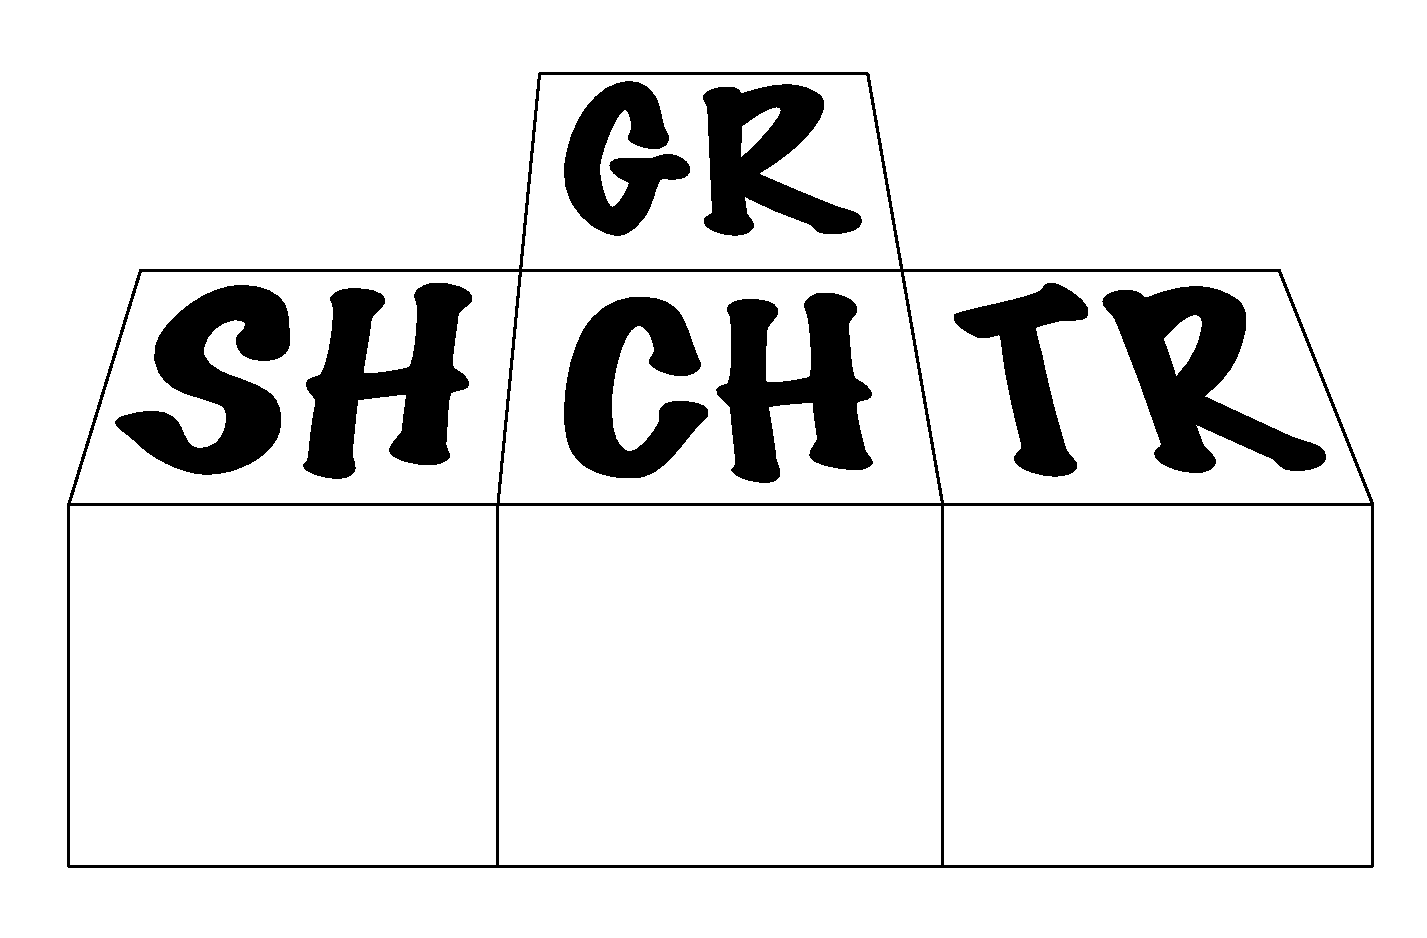
\includegraphics[width=.5\textwidth]{tetrophon.pdf}
	\caption{An example \emph{tetromino} whose phoneme representation is transparent.}
	\label{tet}
\end{figure}

\section{Evaluation of Our Method}
To investigate the effect of interaction in the password generation process, we will isolate two populations of subjects: one group will be aware of the phonemes while playing the game while the other will not have the random phonemes be transparent as an element of the game. After playing, the groups will be asked to memorize a chosen generated password. Both parties will also participate in a memory exercise in attempt to memorize a automatically generated random pronounceable password. We also time the entry of the passwords to effectively study the usability of the passwords generated with the various methods. Participants of this study will be asked to return for follow-up evaluation of password recall. We do not ask the users to produce their own passwords since we feel this would intorduce a hazard in that they may simply prefix or append suffixes to existing live passwords that they may be using actively to achieve better memorability. (??) Lastly, an empirical study on the strength of the passwords will be performed using GPU hashing. We choose a hash function representative of contemporary password storage methods. Strength will be based on how many attempts and how arduous it is to crack the collected passwords.

\section{Timeline}
We expect that a functional prototype should be built by the middle of November at the latest and we attempt to complete this phase as soon as possible to allow as much time as available to perform the studies and consequent analysis. We plan to allot approximately 2 weeks to perform the studies, perhaps completing some analysis concurrently wherever possible (some data may need the full sample size in order to be meaningful). We may feature a mock-interview session (done by members of our team) in a film to showcase the process in an enticing manner. Final report as well as poster and slides will hopefully be done by early December. 

\section{Conclusion}
We have limited time to commit to the studies but we hope our modest incursion into this genre of password generation will spark intrigue and propel further study.


\bibliographystyle{IEEEtran}
\bibliography{IEEEabrv,writeup.bib}
% \begin{thebibliography}{1}
% 	\bibitem{}
% \end{thebibliography}

% that's all folks
\end{document}


